\section{Algoritmos}

Formalmente >qué es un algoritmo? no es una pregunta fácil de responder, de hecho, no daremos una definición formal, apelaremos a la intuición que el alumno tenga hasta el momento.
Intuitivamente podemos decir que un algoritmos es un \emph{método} o \emph{conjunto de instrucciones} que sirven para resolver cierto problema.
La duda que puede surgir es >qué clase de problemas pueden ser resueltos por un algoritmo?
Claramente no existe un método para solucionar el problema del hambre en el mundo, o el problema de cómo una persona puede llegar a fin de mes sin deudas.
Diremos entonces que los problemas que nos interesan son los \emph{problemas computacionales}, más adelante definiremos formalmente qué se entiende por problema computacional.
Por ahora nos limitaremos a decir que un problema computacional se plantea en forma de INPUT y OUTPUT: dada una representación de datos de entrada válida INPUT queremos obtener una representación de datos de salida OUTPUT que depende del INPUT y que cumple ciertas condiciones.
Con estos conceptos podemos decir que un algoritmo es un método para convertir un INPUT válido en un OUTPUT.
>Qué significa que un INPUT sea válido? eso dependerá completamente del problema en cuestión.
A este método le exigiremos ciertas propiedades:
\begin{itemize}
  \itemsep 0pt
  \item[-] Precisión: cada instrucción debe ser planteada en forma precisa y no ambigua.
  \item[-] Determinismo: cada instrucción tiene un único comportamiento que depende solamente del input.
  \item[-] Finitud: el método está compuesto por un conjunto finito de instrucciones.
\end{itemize}

Diremos que las instrucciones del algoritmo se \emph{ejecutan}\footnote{Cuando hablemos de la ejecución de las instrucciones de un algoritmo el sujeto siempre será el algoritmo mismo, diremos que él ejecuta las instrucciones.} y que el algoritmo se detiene si no hay más instrucciones que ejecutar o si ya se produjo un OUTPUT.
Un concepto importantísimo es cuándo consideraremos que un algoritmo es correcto.
En nuestro caso diremos que un algoritmo es correcto si para todo INPUT válido luego de comenzar la ejecución del algoritmo, este se detiene y produce un OUTPUT correcto para el INPUT.
Una implicación importante es que de aquí se deduce cuándo un algoritmo es incorrecto: si existe al menos un INPUT válido para el cuál, o el algoritmo no se detiene, o calcula un OUPUT incorrecto, entonces diremos que el algoritmo es incorrecto.

El alumno debe estar acostumbrado a los ejemplos tipo ``receta de cocina'' muy comentados en cursos introductorios de computación.
Nos evitaremos este tipo de ejemplos e introduciremos nuestra notación de algoritmo con un problema más cercano a lo que nos interesará en este curso.
Para representar un algoritmo usaremos seudo--código, muy parecido a lo que sería un código en un lenguaje como C o Java pero que no se preocupa de problemas de sintaxis y en algunos casos nos permitirá trabajar de manera simple con conjuntos, operaciones matemáticas, etc.

\begin{ejemplo}
Queremos un algoritmo para, dada una secuencia $S=(s_1,s_2,\ldots,s_n)$ de $n$ números enteros de input, genere como output el valor máximo de esa secuencia.
El siguiente es un algoritmo ``iterativo'' que resuelve el problema planteado:
\begin{codebox}
\Procname{INPUT: Una secuencia $S=(s_1,s_2,\ldots,s_n)$ y un natural $n\geq 1$ que representa el largo de la secuencia. \\
OUTPUT: $m=\max\{s_1,s_2,\ldots,s_n\}$, el máximo de los números de la secuencia.

$\proc{Max}(S,n)$}
\li $m\cgets s_1$
\li $k\cgets 2$
\li \While $k\leq n$ \Do
\li \> \If $s_k > m$ \Then
\li \> \> $m\cgets s_k$
\li \> $k\cgets k+1$
\li \Return $m$
\end{codebox}

El siguiente es un algoritmo ``recursivo'' que resuelve el problema planteado:
\begin{codebox}
\Procname{INPUT: Una secuencia $S=(s_1,s_2,\ldots,s_n)$ un natural $n\geq 1$ que representa el largo de la secuencia. \\
OUTPUT: $m=\max\{s_1,s_2,\ldots,s_n\}$, el máximo de los números de la secuencia.

$\proc{Rec-Max}(S,n)$}
\li \If $n=1$ \Then
\li \> \Return $s_1$
\li \Else
\li \> $k:=\proc{Rec-Max}(S,n-1)$
\li \> \If $s_n\geq	k$ \Then
\li \> \> \Return $s_n$
\li \> \Else
\li \> \> \Return $k$
\end{codebox}
\end{ejemplo}

En el ejemplo se han introducido algunas instrucciones que debieran resultar familiares, {\bf while}, {\bf if}--{\bf else}, {\bf return}, que tienen el sentido habitual de un lenguaje de programación de propósito general, hemos usado el operador ``$:=$'' para la asignación, y a veces usaremos también la instrucción {\bf for}.
También se ha introducido la forma de hacer recursión.
Los algoritmos recursivos en general tienen relación directa con definiciones inductivas de objetos (como vimos en la sección 1.1).
Supondremos que el alumno tiene cierta familiaridad también con algoritmos recursivos.
En el algoritmo recursivo anterior se está aprovechando la definición inductiva del máximo de una secuencia de elementos:
\begin{enumerate}
  \itemsep 0pt
  \item $\max\{s_1,s_2,\ldots,s_n\}=\max\{\max\{s_1,s_2,\ldots,s_{n-1}\},s_n\}$
  \item $\max\{s_1\}=s_1$.
\end{enumerate}
En general los algoritmos recursivos se obtendrán casi en forma directa de definiciones inductivas de objetos o propiedades.
 
>Cómo podemos asegurar que los anteriores algoritmos son correctos, o sea, que siempre se detienen y entregan el resultado esperado?
La forma en cómo se diseñaron nos da una intuición de su \emph{corrección}, pero necesitamos métodos más formales para establecer la corrección de un algoritmo.


\subsection{Corrección de Algoritmos}
La herramienta principal que usaremos para demostrar la corrección de los algoritmos será la inducción en sus distintas formulaciones.
Dividiremos nuestro estudio en dos partes, la corrección de algoritmos iterativos y la corrección de algoritmos recursivos.

\subsubsection*{Corrección de Algoritmos Iterativos}
Supongamos que queremos demostrar que un algoritmo no recursivo (o sea, uno en que no hay llamadas recursivas a sí mismo) es correcto. 
La única dificultad proviene de la posibilidad de que el programa contenga \emph{loops}, o sea que realice iteraciones, por lo que nos centramos en este caso\footnote{No nos preocuparán algoritmos no recursivos que no tengan iteraciones ya que en ellos se puede hacer un trazado completo de su ejecución viendo todos los casos y la corrección resulta trivial}.
Generalmente, dividimos la demostración de que un programa iterativo es correcto en dos tareas independientes, que llamamos {\bf corrección parcial} y {\bf terminación} que se definen de la siguiente forma.
Para demostrar la corrección parcial de un algoritmo debemos establecer que, si el algoritmo se detiene, entonces entrega un resultado correcto.
Para la terminación debemos demostrar que el algoritmo efectivamente se detiene.
Introduciremos estos conceptos con un ejemplo.

El siguiente es un algoritmo que recibe como input un par de números naturales $x$ e $y$, analizaremos luego cuál es el output del algoritmo.
\begin{codebox}
\Procname{INPUT: Dos números $x,y\in\N$. \\
OUTPUT: $z=$ ?.

$\proc{M}(x,y)$}
\li $z:=0$
\li $w:=y$
\li \While $w \not= 0$ \Do
\li \> $z:=z+x$
\li \> $w:=w-1$
\li \Return $z$
\end{codebox}

En este algoritmo existe un único \emph{loop}.
Para demostrar la corrección parcial de un algoritmo, lo que generalmente se hace es buscar un {\bf invariante} del \emph{loop}, una expresión lógica que sea verdadera antes de iniciar el \emph{loop} y al final de cada una de las iteraciones del \emph{loop}.
Esta expresión siempre tendrá relación con las variables del algoritmo y generalmente es una expresión que ``une a las variables'', las hace depender unas de otras.
Si encontramos una expresión y logramos demostrar que esta es efectivamente un invariante, entonces esta expresión será verdadera también al finalizar el \emph{loop}, luego de su última iteración, lo que nos permitirá decir que, si el \emph{loop} se detiene entonces la propiedad se cumple.
Dado un \emph{loop} pueden existir muchas propiedades que siempre sean verdaderas antes de iniciar y al final de cada iteración, debemos elegir la que más información nos entregue con respecto a lo que el algoritmo pretende realizar.
Por ejemplo, en el anterior algoritmo está claro que la expresión:
\[
0\leq w\leq y
\]
es un invariante del loop, el problema principal es que no nos dice nada por ejemplo de los valores de las variables $x$ y $z$ que también están participando del algoritmo.

>Cómo buscamos entonces un invariante que nos ayude a demostrar la corrección parcial?
En general debemos centrarnos en buscar propiedades que tengan que ver con lo que queremos que el algoritmo haga.
>Qué hace el anterior algoritmo?
No es difícil notar que el algoritmo anterior, en base a sumas y decrementos, calcula la multiplicación entre $x$ e $y$, por lo que al finalizar el algoritmo se debiera cumplir que $z=x\cdot y$.
Para estar más seguros podemos hacer una tabla con los valores que toman cada variable después de cada iteración.
La siguiente es la tabla mencionada si se supone que los valores de $x$ e $y$ son inicialmente $a$ y $b$, la columna $0$ corresponde a los valores antes de que comience el \emph{loop} y la columna $i$ a los valores al finalizar la $i$--ésima iteración.
\[
\begin{array}{c|ccccccc}
\text{variables} & 0 & 1 & 2 & 3 & 4 & \ldots & b \\ \hline
x & a & a & a &     a  & a  & \cdots & a \\
y & b & b & b &     b  & b  & \cdots & b \\
z & 0 & a & 2a &    3a & 4a & \cdots & b\cdot a \\
w & b & b-1 & b-2 & b-3& b-4& \cdots & 0
\end{array}
\]
El \emph{loop} alcanza a ejecutar $b$ iteraciones luego de lo cuál el valor de $w$ se hace $0$ y se termina con $z=b\cdot a$ que era lo que esperábamos.
Esta tabla nos permite inferir también que la siguiente expresión debiera cierta luego de cada iteración del \emph{loop}:
\[
z=(y-w)x
\]
Si demostráramos que la expresión anterior es un invariante entonces estaríamos seguros que después de la última iteración del \emph{loop} se cumple que $z=(y-w)x$, y dado que el \emph{loop} se detiene sólo si $w=0$ obtendríamos que, si el algoritmo se detiene entonces $z=y\cdot x$.
Para demostrar que $z=(y-w)x$ es un invariante usaremos el principio de inducción simple, en el siguiente lema.

\begin{lema}
La expresión $z=(y-w)x$ es un invariante para el loop del algoritmo $\proc{M}(x,y)$, o sea,
si $x,y\in\N$ y se ejecuta el algoritmo $\proc{M}(x,y)$ entonces luego de cada iteración se cumple que $z=(y-w)x$.

\begin{demostracion}
Las únicas variables que cambian sus valores a medida que el algoritmo se ejecutan son $z$ y $w$, luego hay que centrarse en la evolución de los valores de estas variables.
Sean $z_i$ y $w_i$ los valores que almacenan las variables $z$ y $w$ luego de que se termina la $i$--ésima iteración del algoritmo, $z_0$ y $w_0$ son los valores iniciales.
Demostraremos por inducción que para todo $i$ se cumple que $z_i=(y-w_i)x$.
\begin{inducciondemo}
  \BI Para $i=0$, se tiene que $z_i=z_0=0$ y que $w_i=w_0=y$.
  Ahora, $z_0=0=(y-y)x=(y-w_0)x$ por lo que se cumple que $z_i=(y-w_i)x$ para $i=0$.
  \HI Supongamos que efectivamente se cumple que $z_i=(y-w_i)x$.
  \TI Al final de la iteración $i+1$ el valor de $z$ se ha incrementado en $x$ y el valor de $w$ se ha decrementado en $1$ por lo que se cumple la relación $z_{i+1}=z_i+x$ y $w_{i+1}=w_i-1$.
  Ahora
  \[
  z_{i+1}=z_i+x\stackrel{HI}{=}(y-w_i)x+x=(y-w_i+1)x=(y-(w_i-1))x=(y-w_{i+1})x
  \]
  por lo que la propiedad también se cumple para $i+1$.
\end{inducciondemo}
Por inducción entonces se ha demostrado que después de cada iteración se cumple que $z=(y-w)x$ y por lo tanto si el algoritmo termina, el resultado será $z=y\cdot x$
\end{demostracion}
\end{lema}

Hemos demostrado la corrección parcial del algoritmo, ahora debemos demostrar que el algoritmo efectivamente termina, generalmente esta parte es más simple de demostrar, y casi siempre basta con encontrar una expresión entera que decrezca o se incremente con cada iteración y argumentar que llegado a cierto valor en la sucesión el algoritmo se detendrá
El siguiente lema demuestra la terminación del anterior algoritmo.

\begin{lema}
Si $x,y\in\N$ y se ejecuta el algoritmo $M(x,y)$ entonces este se detiene.

\begin{demostracion}
Note que el valor de $w$ es inicialmente $y\in\N$ y después de cada iteración se decrementa en $1$.
Los valores de $w$ forman entonces una sucesión siempre decreciente de valores consecutivos que se inicia en un número natural, por lo que en algún momento $w$ tomará el valor $0$ (ya que $0$ es el menor de los números naturales) y por lo tanto el \emph{loop} terminará y también el algoritmo.
\end{demostracion}
\end{lema}

Finalmente con los dos lemas anteriores se demuestra directamente el siguiente teorema.

\begin{teorema}
El algoritmo $M(x,y)$ retorna el valor $x\cdot y$ (cuando $x,y\in\N$).

\begin{demostracion}
Directa de los dos lemas anteriores.
\end{demostracion}
\end{teorema}

Podemos usar esta misma estrategia para demostrar que el algoritmo iterativo $\proc{Max}(S,n)$ es también correcto, o sea, que después de ejecutarlo con una secuencia $S$ de valores y un natural $n\in\N$ correspondiente a la cantidad de valores de la secuencia, el algoritmo retorna el máximo de la secuencia $S$.
En el siguiente ejemplo se discuten algunos aspectos de esta demostración.

\begin{ejemplo}
Demostraremos que si el algoritmo $\proc{Max}(S,n)$ del principio de esta sección se ejecuta con una secuencia $S$ de $n$ valores $s_1,s_2,\ldots,s_n$ entonces retorna el máximo de la secuencia.
Nos evitaremos la formalidad de establecer teoremas y lemas para la demostración.

Lo primero es notar que el algoritmo termina, su justificación se deja como ejercicio.
Ahora debemos justificar que si el algoritmo termina calcula el resultado correcto.
Debemos encontrar un invariante del \emph{loop} del algoritmo, una expresión que siempre se mantenga verdadera.
Dado que las únicas variables que se modifican durante la ejecución son $m$ y $k$ debemos encontrar una invariante que incluya a estas dos variables y a los valores de la secuencia $S$.
Proponemos el siguiente invariante: en todo momento se cumple que
\begin{equation} \label{eq:inv-max}
m\in S\text{ y }m\geq s_1,s_2,\ldots,s_{k-1}
\end{equation}
o sea, en todo momento $m$ es mayor o igual a los $k-1$ elementos iniciales de $S$.
Nótese que si demostramos que~(\ref{eq:inv-max}) es efectivamente un invariante entonces, dado que al terminar el algoritmo el valor de $k$ es $n+1$, sabríamos que al terminar el algoritmo $m$ es efectivamente el máximo.
La primera parte del invariante ($m\in S$) es simple de justificar ya que basta mirar el código para notar que cada asignación posible a $m$ es con uno de los valores $s_i$.
La que es un poco más complicada es la segunda parte que la demostraremos por inducción.
Sean $m_i$ y $k_i$ los valores de las variables $m$ y $k$ al finalizar la $i$--ésima iteración del \emph{loop}, por inducción demostraremos que para todo $i$ se cumple que 
\[
m_i\geq s_1,s_2,\ldots,s_{k_i-1}
\]
\begin{inducciondemo}
  \BI Para $i=0$ (o sea antes de comenzar la primera iteración del \emph{loop}) se cumple que $m_i=m_0=s_1$ y que $k_i=k_0=2$, por lo que $m_i=s_1\geq s_1=s_{2-1}=s_{k_i-1}$.
  \HI Supongamos que al final de la iteración $i$ efectivamente se cumple que $m_i\geq s_1,s_2,\ldots,s_{k_i-1}$.
  \TI Al final de la iteración $i+1$ el valor de $k$ se incrementa en $1$ por lo que $k_{i+1}=k_i+1$.
  Ahora el valor de $m$ se modifica dependiendo del resultado del {\bf if} de las líneas 4--5, dependiendo de su comparación con el valor $s_k$.
  Algo muy importante de notar es que al momento de la comparación en el {\bf if}, los valores de $m$ y $k$ que se comparan son los correspondientes a la iteración anterior ($i$ en nuestro caso).
  Tendremos entonces dos casos dependiendo del resultado del {\bf if}: (1) $m_{i+1}=m_i$ si $m_i\geq s_{k_i}$, o (2) $m_{i+1}=s_{k_i}$ si $s_{k_i}>m_{i}$.
  Dividiremos entonces la demostración:
  \begin{itemize}
    \item[(1)] Si $m_i\geq s_{k_i}$, entonces al final de la iteración $i+1$ sabemos que $m_{i+1}=m_i$ y $k_{i+1}=k_i+1$.
    Por HI sabemos que $m_i\geq s_1,s_2,\ldots,s_{k_i-1}$ y como además sabemos que $m_i\geq s_{k_i}$ podemos concluir que $m_i\geq s_1,s_2,\ldots,s_{k_i-1},s_{k_i}$.
    Ahora, dado que en este caso $m_{i+1}=m_i$ obtenemos que
    \[
    m_{i+1}=m_i\geq s_1,s_2,\ldots,s_{k_i-1},s_{k_i}.
    \] 
    Cómo también sabemos que $k_{i+1}=k_i+1$, se cumple que $s_{k_i}=s_{k_{i+1}-1}$, así finalmente obtenemos que
    \[
    m_{i+1}\geq s_1,s_2,\ldots,s_{k_{i+1}-1}
    \] 
    que es lo que queríamos demostrar.
    \item[(2)] Si $s_{k_i}>m_i$, entonces al final de la iteración $i+1$ sabemos que $m_{i+1}=s_{k_i}$ y $k_{i+1}=k_i+1$.
    Por HI sabemos que $m_i\geq s_1,s_2,\ldots,s_{k_i-1}$ y como además sabemos que $s_{k_i}>m_i$  
    obtenemos que $s_{k_i}\geq s_1,s_2,\ldots,s_{k_i-1}$.
    Ahora, dado que en este caso $m_{i+1}=s_{k_i}$ y es claro que $s_{k_i}\geq s_{k_i}$ obtenemos que
    \[
    m_{i+1}=s_{k_i}\geq s_1,s_2,\ldots,s_{k_i-1},s_{k_i}.
    \]
    Cómo también sabemos que $k_{i+1}=k_i+1$, se cumple que $s_{k_i}=s_{k_{i+1}-1}$, así finalmente obtenemos que
    \[
    m_{i+1}\geq s_1,s_2,\ldots,s_{k_{i+1}-1}
    \] 
    que es lo que queríamos demostrar.
  \end{itemize}
  Finalmente la propiedad también se cumple para $i+1$.
\end{inducciondemo}
Por inducción hemos demostrado que~(\ref{eq:inv-max}) es efectivamente un invariante para el algoritmo $\proc{Max}(S,n)$ y que por lo tanto siempre se cumple que $m\in S$ y $m\geq s_1,s_2,\ldots,s_{k-1}$.
Ahora si el algoritmo termina el valor de $k$ es $n+1$ por lo que se cumpliría que 
\[
m\in S\text{ y }m\geq s_1,s_2,\ldots, s_n
\]
y por lo tanto $m$ es el máximo.
Cómo antes demostramos que el algoritmo terminaba, podemos decir que $\proc{Max}(S,n)$ correctamente calcula el máximo de la secuencia $S$.
\end{ejemplo}

%Hay algunos algoritmos que usan a otros como \emph{subrutinas} para demostrar su corrección generalmente lo haremos suponiendo que las subrutinas son correctas.
%En el siguiente ejemplo se muestra un algoritmo que usa a $\proc{Max}(S,n)$ y a una función intercambia$(x,y)$ como subrutinas.
%
%\begin{ejemplo}
%El siguiente es un algoritmo para ordenar una secuencia de números en orden creciente.
%En se utiliza el procedimiento $\proc{Max}(S,n)$ que suponemos que correctamente calcula el máximo de los valores de una secuencia de largo $k$ y la función intercambia$(x,y)$ que luego de ejecutar intercambia los valores de las variables $x$ e $y$.
%\begin{codebox}
%\Procname{INPUT: Una secuencia $S=(s_1,s_2,\ldots,s_n)$ y un natural $n\geq 1$ que representa el largo de la secuencia. \\
%OUTPUT: La secuencia $S$ de entrada ordenada en forma creciente, o sea, luego de la ejecución del algoritmo se cumplirá que $s_1\leq s_2\leq\cdots\leq s_n$.
%
%$\proc{SelectSort}(S,n)$}
%\li $k\cgets n$
%\li \While $k\not=1$ \Do
%\li \> $m\cgets\proc{Max}(S,k)$
%\li \> intercambia$(s_k,m)$
%\li \> $k\cgets k-1$
%\end{codebox}
%\end{ejemplo}

\subsubsection*{Corrección de Algoritmos Recursivos}
Para los algoritmos recursivos generalmente no se hace la división entre corrección parcial y terminación, simplemente se demuestra la propiedad deseada por inducción.
La inducción es en general en función del tamaño del input. 
La hipótesis de inducción siempre dirá algo como ``si el algoritmo se ejecuta con un input de tamaño $i$ entonces es correcto\footnote{correcto en el sentido de que entrega el resultado que efectivamente debiera entregar para un input de tamaño $i$}'', y a partir de esa hipótesis intentamos demostrar que ``si el algoritmo se ejecuta con un input de tamaño $i+1$ también será correcto''.
Obviamente el argumento también se puede plantear por inducción por curso de valores: como hipótesis tomaremos que ``si el algoritmo se ejecuta con un input de tamaño menor que $i$ entonces es correcto'' y a partir de ella intentamos demostrar que ``si el algoritmo se ejecuta con un input de tamaño $i$ también será correcto''.
En cualquier caso siempre se tendrá que tomar en cuenta el caso base por separado.
Mostraremos el método con un ejemplo.

\begin{ejemplo}
Demostraremos que el algoritmo $\proc{Rec-Max}(S,n)$ está correcto, o sea, efectivamente retorna el máximo de una secuencia $S=s_1,s_2,\ldots,s_n$ de largo $n$.
La demostración la haremos directamente por inducción en el tamaño del input, en este caso la inducción se hará en el largo $i$ de la secuencia.
Demostraremos que para todo valor $i$ se cumple que el resultado retornado por $\proc{Rec-Max}(S,i)$ es el máximo de los valores $\geq s_1,s_2,\ldots,s_i$.
\begin{inducciondemo}
  \BI La base en este caso es $i=1$.
  Si se ejecuta $\proc{Rec-Max}(S,i)$ con $i=1$ el resultado será $s_1$ por lo que el resultado será el máximo de la secuencia compuesta sólo por $s_1$ y se cumple la propiedad.
  \HI Supongamos que si se ejecuta $\proc{Rec-Max}(S,i)$ el resultado será el máximo de los valores $s_1,s_2,\ldots,s_i$.
  \TI Queremos demostrar que si se ejecuta $\proc{Rec-Max}(S,i+1)$ el resultado será el máximo de los valores $s_1,s_2,\ldots,s_n,s_{i+1}$.
  Si se ejecuta $\proc{Rec-Max}(S,i+1)$ solo tenemos que preocuparnos de las líneas $4$ en adelante (ya que el $i+1$ no es igual a $1$).
  En la línea 4 se llama a $\proc{Rec-Max}(S,i)$ ($i=(i+1)-1$) que por HI es correcto, o sea, luego de la ejecución de la línea 4, el valor de $k$ será igual al máximo entre los valores $s_1,s_2,\ldots,s_i$.
  Ahora tenemos dos posibilidades, que se ejecute la línea 6 o la línea 8 dependiendo del resultado del {\bf if} de la línea 5:
  \begin{itemize}
    \item[(1)] Si se ejecuta la línea 6, es porque se cumple que $s_{i+1}$ es mayor o igual a $k$, o sea $s_{i+1}$ es mayor o igual al máximo de los valores $s_1,s_2,\ldots,s_i$, luego si esto ocurre, sabemos que $s_{i+1}$ es el máximo de los valores $s_1,s_2,\ldots,s_{i+1}$ y por lo tanto $\proc{Rec-Max}(S,i+1)$ entregaría un resultado correcto, ya que se retorna $s_{i+1}$. 
    \item[(2)] Si se ejecuta la línea 8, es porque se cumple que $s_{i+1}$ es menor estricto que $k$, por lo que el máximo de la secuencia $s_1,s_2,\ldots,s_{i+1}$ sería simplemente $k$, luego $\proc{Rec-Max}(S,i+1)$ entregaría un resultado correcto ya que retorna $k$.
   \end{itemize}
\end{inducciondemo}
Por inducción demostramos que para todo $i$ se cumple que el resultado retornado por $\proc{Rec-Max}(S,i)$ es el máximo de los valores $\geq s_1,s_2,\ldots,s_i$ y por lo tanto $\proc{Rec-Max}(S,i)$ es correcto.
\end{ejemplo}

\subsection{Notación Asintótica}
En la sección anterior estudiamos la corrección de algoritmos que se refería a determinar si un algoritmo es o no correcto.
Sin embargo, a pesar de que un algoritmo sea correcto puede ser poco útil en la práctica porque, al implementar el algoritmo en algún lenguaje de programación de propósito general como C o JAVA, el tiempo necesario para que el algoritmo termine puede ser demasiado alto.
Necesitamos entonces estimaciones del tiempo que le tomará a un algoritmo ejecutar en función del tamaño de los datos de entrada, generalmente, a medida que el tamaño de los datos de entrada crece el algoritmo necesitará más tiempo para ejecutar.
Estas estimaciones deben ser lo más independientes del lenguaje en el que lo implementemos, del compilador que usemos e idealmente independientes de las características del hardware que utilicemos para la ejecución en la práctica.
No nos interesará entonces el tiempo exacto de ejecución de un algoritmo dado, si no más bien el ``orden de crecimiento'' del tiempo necesario con respecto al tamaño del input.
En lo que sigue introduciremos una notación que nos permitirá obtener estimaciones con estas características.

Trataremos con funciones con dominio natural $\N$ y recorrido real positivo $\R^+$.
El dominio representará al tamaño del input de un algoritmo y el recorrido al tiempo necesario para ejecutar el algoritmo, por eso nos interesará $\R^+$ (no tiene sentido hablar de tiempo negativo).

\begin{definicion}
Sean $f:\N\rightarrow\R^+$ y $g:\N\rightarrow\R^+$ funciones con dominio natural y recorrido real positivo.
%\begin{itemize}
	%\item 
	Definimos $O(g(n))$ como el conjunto de todas las funciones $f$ tales que existen $c\in\R^+$ y $n_0\in\N$, que cumplen:
	\[
	\forall n>n_0,\;\;\;\; f(n)\leq cg(n).
	\]
	Cuando $f(n)\in O(g(n))$ diremos que $f(n)$ es \emph{a lo más} de orden $g(n)$, o simplemente que $f(n)$ \emph{es} $O(g(n))$.
	
%	\item 
	Definimos $\Omega(g(n))$ como el conjunto de todas las funciones $f$ tales que existen $c\in\R^+$ y $n_0\in\N$, que cumplen:
	\[
	\forall n>n_0,\;\;\;\; f(n)\geq cg(n).
	\]
	Cuando $f(n)\in \Omega(g(n))$ diremos que $f(n)$ es \emph{a lo menos} de orden $g(n)$, o simplemente que $f(n)$ \emph{es} $\Omega(g(n))$.
%\end{itemize}

  Finalmente definimos $\Theta(g(n))$ como la intersección entre $O(g(n))$ y $\Omega(g(n))$, o sea, como el conjunto de todas las funciones $f$ tales que $f(n)\in O(g(n))$ y $f(n)\in\Omega(g(n))$.
  Definiéndolo de manera similar a los casos anteriores diremos que $\Theta(g(n))$ es el conjunto de todas las funciones $f$ tales que existen $c_1,c_2\in\R^+$ y $n_0\in\N$ que cumplen:
  \[
	\forall n>n_0,\;\;\;\; f(n)\leq c_1g(n)\wedge f(n)\geq c_2g(n).
	\]
  Cuando $f(n)\in \Theta(g(n))$ diremos que $f(n)$ \emph{es (exactamente)} de orden $g(n)$, o simplemente que $f(n)$ \emph{es} $\Theta(g(n))$.
  
  Estos conceptos se ven en la figura~\ref{fig:complexity-notation}.
\end{definicion}

\begin{figure}[h!]
\centering 
\begin{tabular}{ccc}
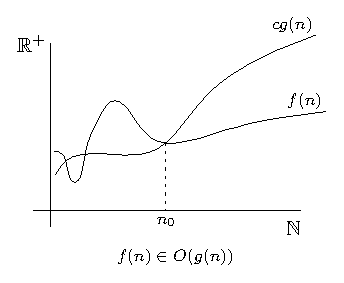
\includegraphics{eps_imgs/O.eps}&
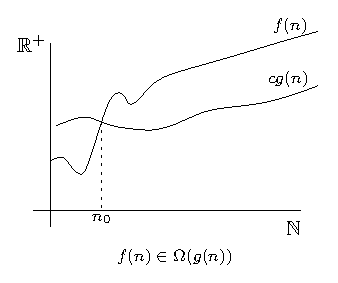
\includegraphics{eps_imgs/Omega.eps}&
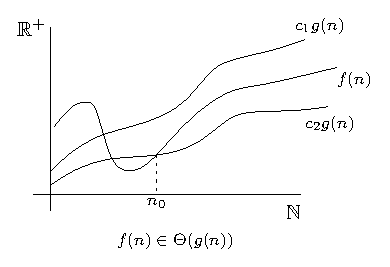
\includegraphics{eps_imgs/Theta.eps}
\end{tabular}
\caption{Órdenes de crecimiento de funciones.}
\label{fig:complexity-notation}
\end{figure}

\begin{ejemplo}
La función $f(n)=60n^2$ es $\Theta(n^2)$.
Para comprobarlo debemos demostrar que $f(n)$ es $O(n^2)$ y $\Omega(n^2)$ simultaneamente.
En el primer caso debemos encontrar $c$ y $n_0$ tal que $\forall n>n_0$ se cumpla que $f(n)\leq cn^2$, es claro que si elegimos $c=60$ y $n_0=0$ tenemos que
\[
\forall n>0,\;\;\;\; f(n)=60n^2\leq 60n^2
\]
y por lo tanto se cumple que $f(n)$ es $O(n^2)$.
En el segundo caso debemos encontrar $c$ y $n_0$ tal que $\forall n>n_0$ se cumpla que $f(n)\geq cn^2$, eligiendo los mismos valores $c=60$ y $n_0=0$ tenemos que
\[
\forall n>0,\;\;\;\; f(n)=60n^2\geq 60n^2
\]
y por lo tanto se cumple que $f(n)$ es $\Omega(n^2)$.
Finalmente concluimos entonces que $f(n)=60n^2$ es efectivamente $\Theta(n^2)$.
\end{ejemplo}

\begin{ejemplo}
La función $f(n)=60n^2+5n+1$ es $\Theta(n^2)$ es $\Theta(n^2)$.
Para comprobarlo debemos demostrar que $f(n)$ es $O(n^2)$ y $\Omega(n^2)$ simultaneamente.
En el primer caso debemos encontrar $c$ y $n_0$ tal que $\forall n>n_0$ se cumpla que $f(n)\leq cn^2$.
Para encontrar estos valores usaremos lo siguiente:
\[
\forall n\geq 1,\;\;\;\;f(n)=60n^2+5n+1\leq 60n^2+5n^2+n^2=66n^2,
\]
esto porque $n^2\geq n\geq 1$ para todo $n\geq 1$, entonces si tomamos $c=66$ y $n_0=1$ obtenemos que $f(n)$ cumple con las condiciones para ser $O(n^2)$.
Ahora si usamos que
\[
\forall n\geq 0,\;\;\;\;f(n)=60n^2+5n+1\geq 60n^2+0+0=60n^2,
\]
ya que $1\geq 0$ y $5n>0$ para todo $n\geq 0$, entonces si tomamos $c=60$ y $n_0=0$ obtenemos que $f(n)$ cumple con las condiciones para ser $\Omega(n^2)$.
Finalmente se concluye que $f(n)$ es $\Theta(n^2)$.
\end{ejemplo}

La moraleja que se puede sacar del primer ejemplo es que las constantes no influyen en la notación $\Theta$.
La moraleja en el segundo ejemplo es que para funciones polinomiales sólo el término con mayor exponente influye en la notación $\Theta$.
Estos conceptos se resumen en el siguiente teorema (cuya demostración se deja como ejercicio).

\begin{teorema}
Si $f(n)=a_kn^k+a_{k-1}n^{k-1}+\cdots+a_2n^2+a_1n+a_0$, con $a_i\in\R$ y tal que $a_k>0$, entonces se cumple que $f(n)$ es $\Theta(n^k)$.

\begin{demostracion}
Ejercicio.
\end{demostracion}
\end{teorema}

\begin{ejemplo}
La función $f(n)=\log_2(n)$ es $\Theta(\log_3(n))$.
Supongamos que $\log_2(n)=x$ y que $\log_3(n)=y$ de esto obtenemos que $2^x=3^y$ por la definición de logaritmo.
Si en esta última ecuación tomamos el $\log_2$ a ambos lados obtenemos:
\[
x=\log_2(3^y)=y\log_2(3),
\]
de donde reemplazando los valores de $x$ e $y$ obtenemos
\[
\log_2(n)=\log_2(3)\log_3(n)
\]
De donde obtenemos que
\[
\begin{array}{l}
\forall n>1,\;\;\;\; \log_2(n)\leq \log_2(3)\log_3(n) \\
\forall n>1,\;\;\;\; \log_2(n)\geq \log_2(3)\log_3(n) \\
\end{array}
\]
Si usamos entonces $c=\log_2(3)$ y $n_0=1$ resulta que $f(n)=\log_2(n)$ cumple las condiciones para ser $O(\log_3(n))$ y $\Omega(\log_3(n))$ simultáneamente y por lo tanto es $\Theta(\log_3(n))$.
\end{ejemplo}

El siguiente teorema generaliza el ejemplo anterior, su demostración se deja como ejercicio.

\begin{teorema}
Si $f(n)=\log_a(n)$ con $a>1$, entonces para todo $b>1$ se cumple que $f(n)$ es $\Theta(\log_b(n))$.

\begin{demostracion}
Ejercicio.
\end{demostracion}
\end{teorema}

Este teorema nos permite independizarnos de la base del logaritmo cuando en el contexto de la notación asintótica.
En adelante para una función logarítmica simplemente usaremos $\Theta(\log n)$ sin especificar la base.
Si necesitáramos la base para algún cálculo generalmente supondremos que es 2.

En el siguiente ejemplo....

\begin{ejemplo}
La función $f(n)=\sqrt{n}$ es $O(n)$ pero no es $\Omega(n)$ (y por lo tanto no es $\Theta(n)$).
La parte fácil es mostrar que $\sqrt n$ es $O(n)$, de hecho dado que 
\[
\forall n\geq 0,\;\;\;\; \sqrt{n}\leq n
\]
concluimos que tomando $c=1$ y $n_0=0$ la función $f(n)=\sqrt{n}$ cumple las condiciones para ser $O(n)$.
Queremos demostrar ahora que $f(n)=\sqrt n$ NO es $\Omega(n)$, lo haremos por contradicción.
Supongamos que efectivamente $f(n)=\sqrt n$ es $\Omega(n)$, o sea, existe una constante $c>0$ y un $n_0\in\N$ tal que 
\[
\forall n>n_0,\;\;\;\; \sqrt n\geq cn.
\]
De lo anterior concluimos que 
\[
\forall n>n_0,\;\;\;\; n\geq c^2n^2\Rightarrow 1\geq c^2n,
\]
de donde concluimos que $c^2<1$ (ya que $n>n_0\geq 0$).... [seguir]
\end{ejemplo}

Las distintas funciones que pertenecen a distintos órdenes de crecimiento (notación $\Theta$, $O$ y $\Omega$), tienen nombres característicos, los más importantes se mencionan en la siguiente tabla, $m$ y $k$ son constantes positivas, $m\geq 0$ y $k\geq 2$.
\begin{center}
\begin{tabular}{llcc} 
Notación & Nombre \\ \hline
$\Theta(1)$ & Constante \\
$\Theta(\log n)$ & Logarítmico \\
$\Theta(n)$ & Lineal \\
$\Theta(n\log n)$ & $n\log n$ \\
$\Theta(n^2)$ & Cuadrático \\
$\Theta(n^3)$ & Cúbico \\
$\Theta(n^m)$ & Polinomial \\
$\Theta(k^n)$ & Exponencial \\
$\Theta(n!)$ & Factorial\\
\end{tabular}
\end{center}

\subsection{Complejidad de Algoritmos Iterativos}
%\subsubsection*{Complejidad de Algoritmos Iterativos}

Nos preguntaremos por el tiempo que tarda cierto algoritmo en ejecutar, este tiempo dependerá del tamaño del input y en general lo modelaremos como una función $T(n)$ con $n$ el tamaño del input.
No nos interesa el valor exacto de $T$ para cada $n$ si no más bien una \emph{notasión asintótica} para ella.
Para \emph{estimar} el tiempo lo que haremos es contar las instrucciones ejecutadas por el algoritmo, en algunos casos puntuales estaremos interesados en contar una instrucción en particular y obtener para ese número una notación asintótica.

\begin{ejemplo}
Consideremos el siguiente trozo de código:
\begin{codebox}
\li \For $i:=1$ \To $n$
\li \> \For $j:=1$ \To $i$ \label{li:comp1-for}
\li \> \> $x:=x+1$ \label{li:comp1}
\end{codebox}
Nos interesa encontrar una notación asintótica para el número de veces que se ejecuta la línea~\ref{li:comp1} en función de $n$, digamos que esta cantidad es $T(n)$.
Si fijamos el valor de $i$, las veces que se ejecuta línea~\ref{li:comp1} está ligada sólo al ciclo que comienza en la línea~\ref{li:comp1-for}, y es tal que, si $i=1$ se ejecuta una vez, si $i=2$ se ejecuta dos veces,$\ldots$ si $i=k$ se ejecuta $k$ veces.
Entonces, dado que el valore de $i$ va incrementándose desde $1$ hasta $n$, obtenemos la expresión
\[
T(n)=1+2+3\cdots +(n-1)+n=\frac{n(n+1)}{2}=\frac{n^2}{2}+\frac{n}{2}
\]
de donde concluimos que la cantidad de veces que se ejecuta la línea~\ref{li:comp1} es $\Theta(n^2)$.
\end{ejemplo}

\begin{ejemplo}
Consideremos el siguiente trozo de código:
\begin{codebox}
\li $j:=n$
\li \While $j\geq 1$ \Do \label{li:comp2-while}
\li \> \For $i:=1$ \To $j$ \label{li:comp2-for}
\li \> \> $x:=x+1$ \label{li:comp2}
\li \> $j:=\lfloor\frac{j}{2}\rfloor$ \label{li:comp2-dec}
\end{codebox}
Nos interesa encontrar una notación asintótica para el número de veces que se ejecuta la línea~\ref{li:comp2} en función de $n$, digamos que esta cantidad es $T(n)$.
En este caso no resulta tan simple el cálculo.
Primero notemos que para un $j$ fijo, las veces que se ejecuta la línea~\ref{li:comp2} está solamente ligada al ciclo {\bf for} que comienza en la línea~\ref{li:comp2-for}.
Ahora cada vez se termina una iteración del ciclo {\bf while} de la línea~\ref{li:comp2-while} el valor de $j$ se disminuye en la mitad.
Supongamos ahora que el ciclo {\bf while} se ejecuta $k$ veces, obtenemos entonces la siguiente expresión para la cantidad de veces que se ejecuta la línea~\ref{li:comp2}:
\[
T(n)=n+\frac{n}{2}+\frac{n}{4}+\cdots+\frac{n}{2^{k-1}}=\sum_{i=0}^{k-1}\frac{n}{2^i}.
\]
Necesitamos una expresión para esta última sumatoria.
Podemos reescribirla y usar la fórmula para la serie geométrica para obtener
\[
\sum_{i=0}^{k-1}\frac{n}{2^i}=n\sum_{i=0}^{k-1}\left(\frac{1}{2}\right)^i=
n\;\frac{1-\left(\frac{1}{2}\right)^k}{1-\frac{1}{2}}=2n\left(1-\left(\frac{1}{2}\right)^k\right).
\]
Ahora, dado que $1-(\frac{1}{2})^k\leq 1$ obtenemos que 
\[
\forall n>1,\;\;\;\;T(n)=\sum_{i=0}^{k-1}\frac{n}{2^i}\leq 2n,
\]
y por lo tanto la cantidad de veces que se ejecuta la línea~\ref{li:comp2} es $O(n)$.
Dado que inicialmente para el valor $j=n$ la línea~\ref{li:comp2} se ejecuta $n$ veces, concluimos que $T(n)\geq n$ y por lo tanto es $\Omega(n)$.
Sumado este último resultado al resultado anterior obtenemos que la cantidad de veces que se ejecuta la línea~\ref{li:comp2} es $\Theta(n)$.
\end{ejemplo}

En los dos ejemplos anteriores hemos visto analizado el número de veces que se ejecuta cierta instrucción con respecto a un parámetro.
Cuando nos enfrentamos a un algoritmo y queremos estimar el tiempo que demora entregando una notación asintótica (como función del tamaño del input) para él, siempre debemos encontrar una o más instrucciones que sean representativas del tiempo que tardará el algoritmo y contar cuántas veces se repite.
Por ejemplo, consideremos el siguiente algoritmo que busca un elemento dentro de una lista
\begin{codebox}
\Procname{INPUT: Una secuencia de enteros $S=s_1,s_2,\ldots, s_n$, un natural $n>0$ correspondiente al largo de la secuencia y un entero $k$. \\
OUTPUT: El índice en el que $k$ aparece en la secuencia $S$ o $0$ si $k$ no aparece en $S$.

$\proc{Búsqueda}(S,n,k)$}
\li \For $i:=1$ \To $n$
\li \> \If $s_i=k$ \Then \label{li:comp3-if}
\li \> \> \Return $i$ \label{li:comp3-ret1}
\li \Return 0 \label{li:comp3-ret2}
\end{codebox}

En este algoritmo por ejemplo, las líneas~\ref{li:comp3-ret1} y~\ref{li:comp3-ret2} no son representativas del tiempo que tardará este algoritmo ya que cada una de ellas o no se ejecuta o se ejecuta sólo una vez.
Resulta entonces que una instrucción representativa es la que se realiza en la línea~\ref{li:comp3-if} más específicamente la comparación que se realiza en~\ref{li:comp3-if}.
Otro punto importante es cómo medimos el tamaño del input.
En este y otros casos en donde el input sea una lista de elementos, será natural tomar como tamaño del input la cantidad de elementos en la lista.
Queremos entonces encontrar una notación $\Theta$ para las veces que se ejecuta la comparación de la línea~\ref{li:comp3-if} en función del parámetro $n$, llamaremos a esta cantidad $T(n)$.
Un problema que surge es que esta cantidad no sólo dependerá de $n$ si no también de cuáles sean los datos de entrada.
Para sortear este problema dividiremos entonces el estudio de un algoritmo en particular en estimar el tiempo que tarda en el \emph{peor caso} y en el \emph{mejor caso} por separado para un tamaño de input específico.
Por peor caso se refiere a la situación en que los datos de entrada hacen que el algoritmo tarde lo más posible, y por mejor caso a la situación en que los datos hacen que se demore lo menos posible.
En nuestro ejemplo, el mejor caso ocurre cuando $s_1=k$ en cuyo caso la línea~\ref{li:comp3-if} se ejecuta una única vez y por lo tanto $T(n)$ es $\Theta(1)$.
En cuanto al peor caso, este ocurre cuando $k$ no aparece en $S$ y por lo tanto la línea~\ref{li:comp3-if} se ejecuta tantas veces como elementos tenga $S$, o sea $T(n)$ es $\Theta(n)$.
Diremos finalmente que el algoritmo $\proc{Búsqueda}(S,n,k)$ es de \emph{complejidad} $\Theta(n)$ en el peor caso y $\Theta(1)$ en el mejor caso.

Tomemos el siguiente ejemplo para analizar también el mejor y peor caso.

\begin{ejemplo}
Consideremos el siguiente algoritmo para ordenar una secuencia de números enteros.
\begin{codebox}
\Procname{INPUT: Una secuencia de enteros $S=s_1,s_2,\ldots, s_n$, un natural $n>0$ correspondiente al largo de la secuencia. \\
OUTPUT: Al final del algoritmo la secuencia $S$ se encuentra ordenada, es decir $s_1\leq s_2\leq\cdots \leq s_n$.

$\proc{Insert-Sort}(S,n)$}
\li \For $i:=2$ \To $n$ \label{li:comp4-for}
\li \> $t:=s_i$
\li \> $j:=i-1$
\li \> \While $s_j>t\;\wedge j\geq 1$ \Do \label{li:comp4-while}
\li \> \> $s_{j+1}:=s_j$ \label{li:comp4-asig}
\li \> \> $j:=j-1$ \label{li:comp4-dec}
\li \> $s_j:=t$
\end{codebox}

Este algoritmo para cada iteración $i$ del ciclo principal, busca la posición que le corresponde a $s_i$ en la secuencia ya ordenada $s_1,s_2,\ldots,s_i$ y lo ``inserta'' directamente en la posición que corresponde ``moviendo'' los valores que sean necesarios.
La búsqueda del lugar mas el movimiento de los valores se hacen en el ciclo que comienza en la línea~\ref{li:comp4-while}.
El alumno como ejercicio puede demostrar la corrección de este algoritmo, o sea que efectivamente ordena la secuencia $S$.

En este caso las instrucciones representativas para calcular el tiempo $T(n)$ que demora el algoritmo en ordenar una secuencia de largo $n$, son las que se encuentran en el ciclo que comienza en~\ref{li:comp4-while}.
El mejor caso del algoritmo ocurre entonces cuando el ciclo en~\ref{li:comp4-while} ni siquiera comienza, o sea en el caso que cada vez que se llegue a él, se cumpla que $s_j\leq t$, o sea que $s_{i-1}\leq s_i$ para $2\leq i\leq n$, es decir, el mejor caso ocurre cuando la secuencia inicialmente está ordenada, en este caso la comparación de la línea~\ref{li:comp4-while} se repite $n-1$ veces y por lo tanto $T(n)$ es $\Theta(n)$ en el mejor caso.
El peor caso ocurre cuando el ciclo en~\ref{li:comp4-while} se detiene porque $j<1$ en este caso el ciclo de la línea $i-1$ veces para cada valor de $i$ entre $2$ y $n$, por lo tanto una estimación para $T(n)$ estaría dada por la expresión
\[
1+2+\cdots + (n-1)=\frac{n(n-1)}{2}
\]
que sabemos que es $\Theta(n^2)$.
Finalmente diremos que el algoritmo $\proc{Insert-Sort}(S,n)$ tiene complejidad $\Theta(n^2)$ en el peor caso y $\Theta(n)$ en el mejor caso.
\end{ejemplo}

En computación estamos interesados principalmente en el peor caso de ejecución de un algoritmo, ya que esto nos dará una estimación de qué tan mal puede comportarse el algoritmo en la práctica.
A veces puede resultar difícil encontrar una notación $\Theta$ ($O$ y $\Omega$ a la vez) para un algoritmo, por lo que nos conformaremos con una buena aproximación $O$ (tanto para el mejor como peor caso) que también nos dará una cota superior al tiempo total usado por el algoritmo.

Un punto importante en el que no hemos puesto suficiente énfasis es en cómo medimos el tamaño del input para un algoritmo.
Mencionamos que cuando consideremos el input como una lista de elementos usaremos como tamaño del input la cantidad de elementos de la lista, esto principalmente porque las operaciones que se harán serán comparaciones o intercambios de valores entre los elementos de la secuencia.
En el siguiente ejemplo el algoritmo recibe un único elemento y decide si es o no un número primo.
\begin{codebox}
\Procname{INPUT: Un número natural $n>1$. \\
OUTPUT: {\bf SI} si $n$ es un número primo, {\bf NO} en otro caso. 

$\proc{EsPrimo}(n)$}
\li \For $i:=2$ \To $n-1$ \label{li:comp5-for}
\li \> \If  $\;n$ mod $i=0$ \Then \label{li:comp5-if}
\li \> \> \Return NO
\li \Return SI
\end{codebox}

En este caso podemos estimar el tiempo en función de las veces que se ejecute la línea~\ref{li:comp5-if}.
Es claro que el mejor caso es que el valor $n$ sea par, en cuyo caso será inmediatamente divisible por $2$ y el algoritmo toma tiempo $\Theta(1)$.
El peor caso para el algoritmo es cuando $n$ sea efectivamente un número primo.
Si tomáramos el tamaño del input como el valor numérico de $n$ entonces podríamos decir que en el peor caso este algoritmo tarda $\Theta(n)$ que es exactamente la cantidad de veces que se ejecuta el ciclo de la línea~\ref{li:comp5-for}.
Sin embargo, cuando el input es un número $n$, el valor numérico no es una buena estimación del tamaño del input.
Una mucho mejor estimación del tamaño del input, y la que usaremos en el caso de algoritmos numéricos, es la cantidad de dígitos que son necesarios utilizar para representar a $n$.
Si $d$ es la cantidad de dígitos necesaria para representar a $n$, $d$ es aproximadamente $\log_{10}(n)$, y por lo tanto $n$ es aproximadamente $10^d$.
Esto nos lleva a concluir que si el tamaño del input es $d$ (la cantidad de dígitos de $n$) el algoritmo en el peor caso tarda $\Theta(10^d)$, o sea exponencial.
Resulta entonces que el comportamiento del algoritmo es lineal con respecto al valor numérico del input pero exponencial con respecto a la cantidad de dígitos del input.
No lo hemos mencionado aun, pero un tiempo exponencial es muy malo en la práctica, tocaremos este tema en la siguiente sección.

El que el tiempo se mida en cuanto al valor numérico o a la cantidad de dígitos hace diferencias muy importantes en la práctica.
Por ejemplo, una mejora que se puede hacer al algoritmo $\proc{EsPrimo}$ es cambiar el ciclo de la línea~\ref{li:comp5-for} para que sólo revise los valores hasta un umbral de $\sqrt n$ (>por qué funciona?), >cómo afecta esto a la complejidad asintótica del algoritmo?.
Si medimos el tamaño del input como el valor de $n$ vemos que el tiempo se disminuye a $\Theta(\sqrt n)$ que es bastante mejor que $\Theta(n)$.
Sin embargo si tomamos a $d$, la cantidad de dígitos de $n$, como el tamaño del input, por lo que $\sqrt n=n^\frac{1}{2}$ es aproximadamente $10^{\frac{d}{2}}$.
Ahora es posible demostrar que $10^{\frac{d}{2}}>3^d$ por lo que el tiempo de ejecución del algoritmo sería $\Omega(3^d)$ o sea sigue siendo exponencial y, como veremos en la siguiente sección, en la práctica no es mucho lo que ganamos con disminuir el espacio de búsqueda hasta $\sqrt n$.

%Por ahora veremos como esto afecta a una mejora en cuanto al tiempo de ejecución que se le puede hacer al algoritmo anterior.

%Es fácil si pensamos en el tamaño del input como las unidades de espacio que necesita un computador para almacenarlo, más especificamente, la cantidad de bits necesarios
%En algunos casos el input será sólo un valor numérico y el algoritmo aplicará operaciones

En el siguiente ejemplo también se trata el tema de cómo medimos el tamaño del input para un algoritmo.

\begin{ejemplo}
El siguiente algoritmo calcula la representación en base $3$ de un número en base decimal.
Usa una secuencia de valores $s_i$ donde almacena los dígitos en base $3$
\begin{codebox}
\Procname{INPUT: Un número natural $n>1$. \\
OUTPUT: muestra una lista con los dígitos de la representación en base 3 de $n$.

$\proc{Base3}(n)$}
\li $s_1:=0$
\li $j:=1$
\li $m:=n$
\li \While $m>0$ \Do \label{li:comp5-while}
\li \> $s_j:=n$ mod $3$
\li \> $m:=\lfloor\frac{m}{3}\rfloor$
\li \> $j:=j+1$
\li {\bf print} $s_{j-1},s_{j-2},\ldots,s_1$
\end{codebox}
No discutiremos en detalle el por qué este algoritmo es correcto, dejaremos esta discusión como ejercicio y nos centraremos en la complejidad del algoritmo.
El valor de $m$ se va dividiendo por $3$ en cada iteración del ciclo en la línea~\ref{li:comp5-while}, por lo que en la iteración $j$, el valor de $m$ es aproximadamente $n/3^j$.
El ciclo termina cuando el valor de $m$ es 0, o sea cuando $j$ es tal que $n/3^j<1$, o sea $j>\log_3 n$, por lo que el ciclo se ejecuta al menos $\log_3 n$ veces.
Si tomamos el tamaño del input como el valor numérico de $n$ obtenemos que el algoritmo tarda $O(\log n)$, o sea tiempo logarítmico.
Si por otra parte tomamos como tamaño del input la cantidad $d$ de dígitos decimales de $n$, el algoritmo tarda $O(d)$, o sea tiempo lineal.
\end{ejemplo}

\subsection{Relaciones de Recurrencia y Complejidad de Algoritmos Recursivos}
[...falta completar...]


